\section{\gls{dft}}
The \gls{dft} is a mathematical transformation used to analyse the internal periodicities of a time sequence of data. Specifically, it decomposes a periodic time series as a sum of sine waves at different frequencies, giving information on the amplitude and phase of each frequency present in the signal. The more data available, the more detailed \gls{dft} will be.

\noindent This procedure, known as spectral analysis, makes it possible to study signals, waves, vibrations, sounds and images. In addition to these areas, DFT also has major scientific applications, such as the precise estimation of sunspot cycles, helping to predict and control phenomena such as geomagnetic storms\footnote{For more about geomagnetic storms and them correlation with sunspot, see \url{https://en.wikipedia.org/wiki/Geomagnetic_storm}}.

\subsection{Insights}
The \gls{dft} comes about as a discrete version of the \gls{cft}, which represents a continuous function as a potentially infinite sum of sine waves. More rigorously, given a function $f\in L^1\left(\mathbb{R}\right)$ (i.e., a function integrable over the whole $\mathbb{R}$), its Fourier transform is a functional operator, denoted by $\mathcal{F}$, which associates the function $f$ with its frequency representation:
\[
\mathcal{F}(f): \omega \mapsto \int_{\mathbb{R}} e^{-i2\pi \omega x}f(x)\,dx
\]
The \textbf{Fourier inversion theorem} states that, if both $f$ and $\mathcal{F}(f)$ belong to $L^1(\mathbb{R})$ (i.e. they are both integrable), then for almost any $x\in\mathbb{R}$ it is possible to recover $f(x)$ via the following inverse relation:
\[
f(x)=\int_{\mathbb{R}}{\mathcal{F}\left(f\right)}(\omega)e^{i2\pi x\omega}\,d\omega
\]
In other words, the Fourier transform and its inverse allow switching back and forth between the time (or space) and frequency domains.

\bigskip
The discrete version of this transform, namely \gls{dft}, is used to analyse signals sampled at regular intervals. Thus, while \gls{cft} works on continuous signals, \gls{dft} applies to finite and discrete signals, making it suitable for digital signal processing.

\noindent To better understand how \gls{dft} gives information about the amplitudes and phases of the different frequencies that make up a sequence, it is useful to introduce the Fourier coefficients. These coefficients make it possible to decompose a data sequence into sinusoids associated with different frequencies.
\begin{definition}
	We define Fourier coefficients of the sequence $(x_n)_{n=0}^{N-1}$ as those complex numbers $(X_k)_{k=0}^{N-1}$ such that:
	\begin{equation}
		x_n = \frac{1}{N}\sum_{k=0}^{N-1} X_k e^{i2\pi\frac{k}{N}n}
	\end{equation}
\end{definition}

\noindent The $k$-th coefficient gives information about the amplitude and phase of the frequency $\frac{2pi}{N}k$. We present some examples to better understand the meaning of the Fourier coefficients.
\begin{exempli_gratia}
	Take as our first example a time series consisting of $N$ complex numbers, described by the following coefficients:
	\[
		X_0=0,\;X_1=A,\;X_2=0\;\cdots\;X_{N-2}=0,\;X_{N-1}=A
	\]
	From these coefficients we obtain the time series:
	\[
		x_n = \frac{1}{N}A\left(e^{i2\pi \frac{n}{N}} + e^{i2\pi \frac{n}{N}(N-1)}\right) = \frac{2A}{N}\cos\left(2\pi\frac{n}{N}\right)
	\]
	We note that the series is purely periodic, with amplitude $\frac{2A}{N}$ and frequency $\frac{2\pi}{N}$.

	\bigskip
	\noindent Let us now consider a series of different coefficients, where all values are zero except:
	\[
		X_p=A,\;X_{N-p}=A
	\]
	The generated time series will be:
    \[
		x_n = \frac{1}{N}A\left(e^{i2\pi \frac{n}{N}p} + e^{i2\pi \frac{n}{N}(N-p)}\right) = \frac{2A}{N}\cos\left(2\pi\frac{n}{N}p\right)
	\]
	As can be seen, the coefficients refer to the amplitude of a certain frequency. In addition, to obtain a real time series, symmetry on the coefficients is required.

	\bigskip
	\noindent At last, let us see how to derive the phase from a time series. Let us consider the following coefficients:
	\[
		X_0=0,\;X_1=Ae^{i\theta},\;X_2=0,\;\dots,\;X_{N-2}=0,\;X_{N-1}=Ae^{-i\theta}
	\]
	The resulting time series will be:
    \[
		x_n = \frac{2A}{N}\cos\left(\frac{2\pi}{N}n + \theta\right)
	\]
	Here, the modulus of the coefficient describes the amplitude of the frequency, while its argument $\theta$ describes its phase. Again, to ensure that the series is real, the opposite coefficient must be the conjunct of $X_1$.
\end{exempli_gratia}

\bigskip
We now ask ourselves whether it is possible to estimate the Fourier coefficients from a time series.
\begin{proposition} \label{prop:dft_unitaria}
	The matrix $\frac{1}{\sqrt{N}}\left(e^{i2\pi\frac{k}{N}n}\right)_{n,k=0}^{N-1}$ is unitary.
	\begin{proof}
		We prove the thesis by studying the scalar product between two rows of the matrix, one of which is hermitian
		\[
		\frac{1}{N}\sum_{k=0}^{N-1} e^{i2\pi\frac{k}{N}n}\cdot e^{-i2\pi\frac{k}{N}m} = \frac{1}{N}\sum_{k=0}^{N-1} e^{i2\pi\frac{k}{N}(n-m)}
		\]
		If $n = m$, the result of the sum is $1$. Else if $n \neq m$, we optain:
		\[
			\frac{1}{N}\sum_{k=0}^{N-1} e^{i2\pi\frac{k}{N}(n-m)} = \frac{1}{N}\frac{e^{i2\pi\frac{N}{N}(n-m)}-1}{e^{i2\pi\frac{1}{N}(n-m)}-1} = 0
		\]
		This prove that the matrix is unitary.
	\end{proof}
\end{proposition}

\bigskip
Proving that the matrix $\frac{1}{\sqrt{N}}(e^{i2\pi\frac{k}{N}n})_{n,k=0}^{N-1}$ is unitary is extremely relevant to the computation of Fourier coefficients.
\begin{theorem}[\gls{dft}]
	The Fourier coefficients of the time series $(x_n)_{n=0}^{N-1}$ are given by the formula:
	\begin{equation}
		X_k = \sum_{n=0}^{N-1} x_n e^{-i2\pi\frac{n}{N}k}
	\end{equation}
	\begin{proof}
		Define $U$ as matrix $\frac{1}{\sqrt{N}}(e^{i2\pi\frac{k}{N}n})_{n,k=0}^{N-1}$

		\noindent By definition of the discrete Fourier transform, we can write $\vec{X} = \frac{1}{\sqrt{N}}U\vec{x}$, where $\vec{X}$ is the vector of Fourier coefficients and $\vec{x}$ is the vector of the original time series.

		\noindent As shown in \cref{prop:dft_unitaria}, the matrix $U$ is unitary, so it admits an inverse, which is its transposed conjugate $U^H$. \\
		Therefore, we can invert the transformation and obtain:
		\[
			\vec{x} = \sqrt{N}U^H\vec{X}
		\]

		\noindent This relation allows us to get the Fourier coefficients from the time series.
	\end{proof}
\end{theorem}

\subsection{Implications}
The possibility of calculating Fourier coefficients directly by means of a simple matrix-vector product not only makes the analysis very informative, but also easily achievable.

\paragraph{\gls{fft}} The computational cost of the matrix-vector product for computing Fourier coefficients is $O(N^2)$, which is not excessive in itself. However, there is a specific algorithm for Fourier series that reduces this cost to $O(N\log{N})$, comparable to a sorting algorithm. This algorithm, named \gls{fft}, was designed by Cooley and Tukey.

\begin{algorithm}[h]
	\caption{FFT Cooley-Tukey}
	\begin{algorithmic}[1]
		\Procedure{FFT}{$x$}
		\If{$N$ is $1$}
			\Return $x$
		\EndIf

		\State $\text{even} \gets \Call{FFT}{\left[x_0,x_2,\cdots, x_{N-2}\right]}$
		\State $\text{odd} \gets \Call{FFT}{\left[x_1,x_3,\cdots, x_{N-1}\right]}$

		\State $X$ is an array of size $N$

		\For{$k\in 0,\dots,\frac{N}{2}-1$}
			\State $t \gets \exp\left(-2\pi i k / N\right)\cdot \text{odd}[k]$
			\State $X[k] \gets \text{even}[k] + t$
			\State $X[k + N/2] \gets \text{even}[k] - t$
		\EndFor
		\EndProcedure
	\end{algorithmic}
	\label{alg:fft}
\end{algorithm}

\noindent It is possible to further optimise this algorithm using \gls{gpu}, which exploit the high parallelism of processors to further reduce the computational cost. Although \cref{alg:fft} seems to be able to achieve a cost of $O(\log{N})$, there are physical limitations of the \gls{gpu} and in data structures that make its execution very fast, but asymptotically it remains of cost $O(N\log{N})$.

\paragraph{Periodogram} A periodogram graphically represents the amplitude of the different frequencies that make up a time series, highlighting the dominant components of the frequency spectrum. This tool is particularly useful for distinguishing between noise and the significant frequencies of a signal. For example, in the fields of climatology and astrophysics, it is often used to identify periodic cycles in data.

\noindent We see an application of \gls{dft} on the \texttt{sunspots} dataset from the \gls{r} package, which contains the number of sunspots observed each month from $1700$ to $1988$. Sunspots are correlated with the Sun's magnetic activity and one of the goals of the analysis is to identify any periodic cycles in the data.

\begin{center}
	\centering
	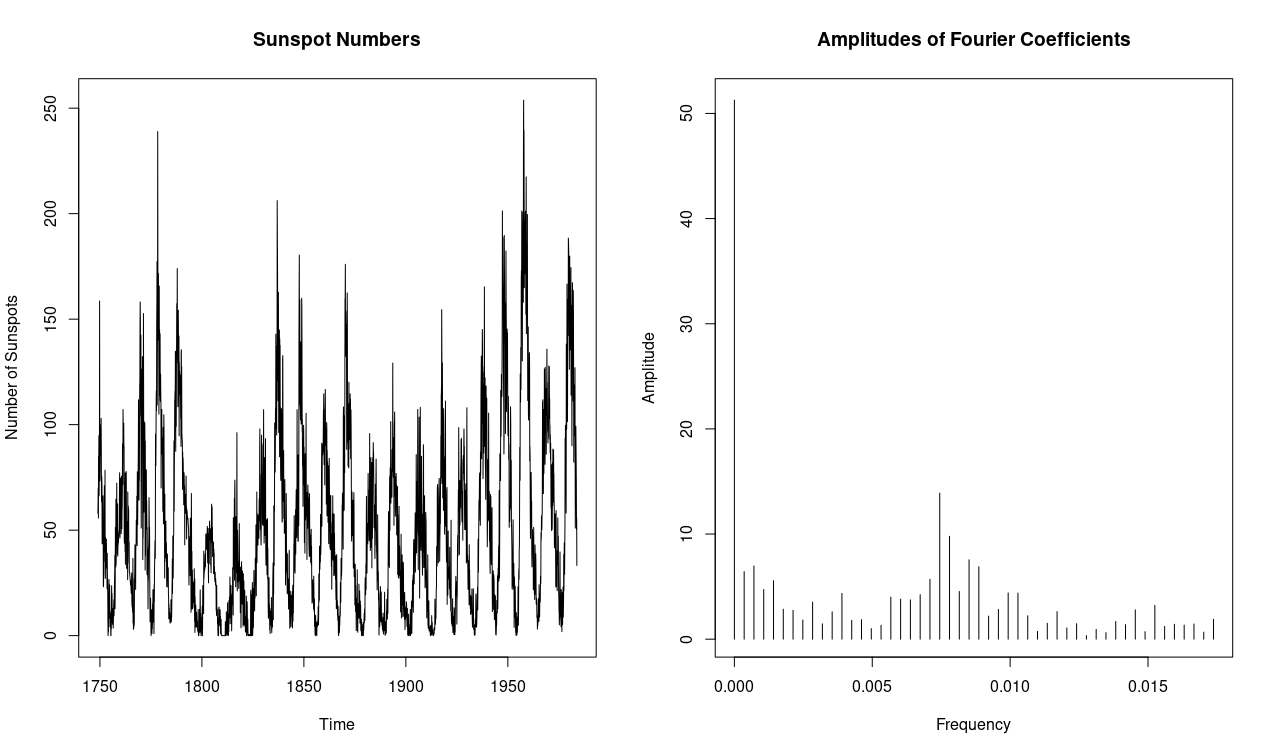
\includegraphics[width=\textwidth]{Figures/sunspots.png}
\end{center}

\noindent Looking at the periodogram obtained with \gls{fft}, we observe that some frequencies are much more pronounced than others. In particular, the frequency $\approx 0.0075\operatorname{\mathrm{Hz}}$ (corresponding to about a cycle of $135$ months) indicates a cycle of about $11$ years, which confirms what is already known about the cyclic nature of solar activity.

\noindent This example demonstrates how the DFT is a powerful tool for detecting and analysing periodic patterns in observational data. The use of the periodogram not only makes it possible to identify the main frequencies, but also to evaluate their relative importance respect to the background noise.
